% !TeX encoding = UTF-8

%\documentclass{LTHtwocol} % Use this when you work on your report.
\documentclass[final]{LTHtwocol} % Use this for the final version.
                                   % It will remove page numbers and
                                   % markers for overfull boxes.
                                   % There really shouldn't be any of those anyway.

\usepackage[utf8]{inputenc}        
\usepackage{amsmath,amssymb,graphicx}
\usepackage{graphicx}  
\usepackage{float} 
\usepackage{xcolor}
\usepackage{hyperref} 
\usepackage{mathrsfs}
\usepackage{listings}                               %Ability to insert code
\usepackage{comment}
\hypersetup{
	colorlinks,
	linkcolor={red!50!black},
	citecolor={blue!50!black},
	urlcolor={blue!80!black}
}

% \usepackage{kantlipsum} % Only for the dummy text. Remove for your own report.

\addbibresource{bibliography.bib}

% Document begins here
\begin{document}
\begin{frontmatter}
\title{Collaborative Robot Trajectory Correction} % Title of the project.

\author[yixi]{Yixi Cai}
\author[yuhan]{Yuhan Xie}
\author[meghan]{Meghan Young}
\author[simon]{Simon Ågren}

\email[yixi]{yi1077ca-s@student.lu.se}
\email[yuhan]{yu1175xi-s@student.lu.se}
\email[meghan]{me3716yo-s@student.lu.se}
\email[simon]{mas15sag@student.lth.se}

\advisor{Julian Salt}

\begin{abstract}
In this work, an autonomous trajectory correction system based on Model Predictive Control (MPC) is realised. The methodology to design and execute this MPC controller on an industrial robot arm with seven degrees of freedom is presented. This system is implemented using a multi-thread code structure to handle trajectory generation and communication of command instructions to the robot simultaneously. The proposed real-time trajectory planning method is shown to succeed in trajectory correction under external perturbations.

\end{abstract}

\end{frontmatter}

% Stick to the proposed structure below. 
% Introduction, Modeling, Electro-Mechanics, Control, Results, Discussion
% Add \subsections{} as appropriate.
% This file compiles on the Automatic Control Department system by typing the
% following into the terminal (while in the directory of the file, and with all
% other files belonging to the template untouched):
% > pdflatex template        
% > biber template
% The first line compiles the .tex file. The second line generates the
% bibliography. Once this is done, you may need to run the first line 1-2
% additional times, for the system to get all cross references right in the
% produced pdf output.

 %\section*{Abbreviation/variable guide, temporary}
 % \begin{itemize}
 %   \item Model predictive control - MPC, except first use in abstract and introduction
 %   \item sample time/period - h
 %   \item the collaborative robot - "Panda"/"the robot"
  %  \item the control interface - (Franka Emika) control interface
 %   \item a time step - k, k+1, ...
 %   \item prediction horizon - N
  %  \item states - x
  %  \item states for MPC - $\zeta$
 %   \item input/ control signal - u
 %   \item controlled variable - z
 %   \item cost function - $J$
%\end{itemize}

\section{Introduction}
%%% Need to improve (also the abstract) after complete other parts %%

% 1 Project Outcome
% improve to be a More general description. 
In this project, the Franka Emika Panda robotic arm, see Figure \ref{fig:Franka}, is required to move between a starting joint configuration and a target joint configuration within a given time. It must be able to complete this task even with perturbations (e.g., manually pushing the robot arm). A model predictive control (MPC) based trajectory generation method is proposed, where a new optimal reference trajectory is calculated every 10 ms. This calculation is performed based on the robot’s new position, thus enabling external disturbances to be handled. Command instructions based on this optimal trajectory are then communicated to the robot. A multi-threaded code structure is used to allow the trajectory calculation and communication to run at the same time.
<<<<<<< HEAD
=======

%The performance of the methodology is verified on the robot arm and (hopefully) shows a satisfying control accuracy. %<-- Not completed yet %<-- Now this is completed :)
>>>>>>> f604414f387b8ccc24728783384143945bbc4ad1

% 2 Outline
The structure of the paper is organized as follows. 
In Section \ref{sec:modeling}, the linear model of the robotic dynamics is constructed in a state-space representation of both continuous-time and discrete-time after a brief analysis of the selection of coordinates.  
In Section \ref{sec:framework}, the equipment and the framework are introduced, providing a general understanding of the project. 
Section \ref{sec:control} demonstrates the design of the MPC controller, followed by the code structure and concrete implementation of the trajectory planning. The function optimized in the MPC controller is proven convex in Appendix \ref{apx:proof}.
In Section \ref{sec:simulation}, the controller and its code is verified. The final implementation and setup leading to the result are presented in Section \ref{sec:experiment}.
The performance of the controller is shown in Section \ref{sec:Results} and later discussed in Section \ref{sec:Conclusion}. Additionally, conclusions are drawn and some possible extension of the project is presented.

% 3 Previous Work
This project and report are heavily based on the 2019 and 2015 papers on real-time point-to-point trajectory generation by Ghazaei, M., Olofsson, B., Robertsson, A. and Johansson, R. \cite{MPC2019} \cite{MPC2015}. The approach, method, and implementation are derived from the papers and applied to the Franka Emika Panda collaborative robotic arm with seven degrees of freedom \cite{frankaweb}.

\begin{figure}[t]
	\centering
	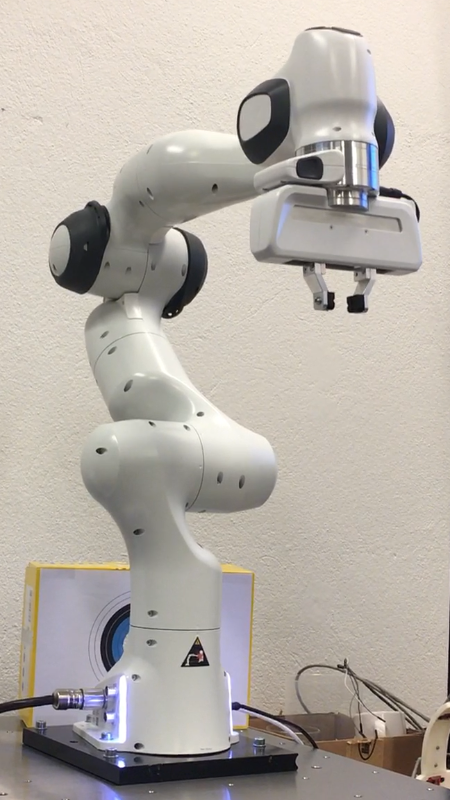
\includegraphics[width=0.5\linewidth]{OurFranka.png}
	\caption{The Franka Emika Panda robot used in the project setup.}
	\label{fig:Franka} 
\end{figure}

\section{Modeling} \label{sec:modeling}
% Generally, the dynamics of the robot arm can be described in any set of generalized coordinates. In applications, Cartesian coordinates and joint coordinates are the most frequently-used coordinates. The Cartesian coordinates have a benefit of simplifying the process in task space but lead to the problem of nonlinearity. Therefore, joint coordinates are applied in this project to describe the system dynamics for the simplification of modeling. It is clear that the motions of each joint are independent and linear under the joint coordinates thus the model can be obtained directly from modeling each joint separately on the form of state-space representation. % Julian: Why clear
%%% A sentence for starting/ Introduction: the meaning of modeling
Derived from physical equations, modeling reveals the structure of a system and gives a causal relationship between control inputs and controlled variables. Generally, the motion of the robot arm can be described in any set of generalized coordinates. A good choice of coordinate can simplify the system equations for certain usage. In applications, Cartesian coordinates and joint coordinates are the most frequently-used coordinates. Joint coordinates are applied for the following considerations:
\begin{enumerate}
    \item The control model input in this project is angular jerk;
    \item The motion can be directly specified in terms of each joint's angle, angular velocity, or higher order time derivatives of the angle under joint coordinates.
\end{enumerate}
Therefore, a linear model for usage of a linear MPC framework can be easily obtained under joint coordinates. Assuming a good tracking performance for the robot, a simple robot model using only the joint kinematic variables can be constructed by decoupled chains of integrators. The state vector is chosen as 
\begin{equation}
    x = [q_1, \dot{q}_1, \Ddot{q}_1, \dots, q_d, \dot{q}_d, \Ddot{q}_d]^T,
\end{equation}
where $q_i$ denotes the angle of i-th joint and $d$ denotes the number of Degrees of Freedom (DoF), i.e., the number of joints, which in this case is equal to 7.

% Typically, the control input can be a dynamic quantity such as force, torque or jerk. In the following description, $u(t)$ represents the jerk inputs of each joint.
\subsection{Continuous-time Model}
A continuous-time linear model is assumed of the form 
\begin{equation}
    \begin{split} 
        \dot{x}(t) & = Ax(t) + Bu(t) \\
        y(t) & = Cx(t),
    \end{split}
\end{equation}
where each joint is modelled as a triple integrator
\begin{equation}
    \Tilde{A} = \begin{bmatrix} 
        0 & 1 & 0 \\
        0 & 0 & 1 \\
        0 & 0 & 0
    \end{bmatrix}, \quad
    \Tilde{B} = \begin{bmatrix}
        0 \\ 0 \\ 1
    \end{bmatrix},
\end{equation}
where the first, second and third state correspond to angular position, velocity and acceleration of the joints respectively; and the input is torque. Assembly of these result in the system matrices\footnote{blkdiag() forms a block diagonal matrix from the given list of matrices.}:
\begin{equation}
    \label{eq:cont-time_model}
    A = \textrm{blkdiag}([\Tilde{A}, \dots, \Tilde{A}]), \quad
    B = \textrm{blkdiag}([\Tilde{B}, \dots, \Tilde{B}]),
\end{equation}
with the dimensions $A\in \mathbb{R}^{3d\times 3d}$ and $B\in \mathbb{R}^{3d\times d}$. The output matrix $C$ is assumed to be the identity matrix with dimension $C\in \mathbb{R}^{3d\times 3d}$, i.e. all states are observable via the control interface. 
% The direct term $D$ was assumed to be $0$.

\subsection{Discrete-time Model}
\label{sec:discretization}
A discrete-time model can be obtained from the continuous-time model on the form of \eqref{eq:cont-time_model} by a first order hold with the sampling period \textit{h} \cite{Wittenmark}. This results in the system 
\begin{equation}
    \label{eq:discr-time_model}
    \begin{split}
        x(k+1) & = \Phi x(k)+\frac{1}{h}\Gamma_1u(k+1) + (\Gamma-\frac{1}{h}\Gamma_1)u(k) \\
        y(k) & = Cx(k),
    \end{split}
\end{equation}
where $\Phi, \Gamma$ and $\Gamma_1$ are given by
\begin{equation}
    \begin{bmatrix} \Phi & \Gamma & \Gamma_1 \end{bmatrix} 
    = \begin{bmatrix} I & 0 & 0 \end{bmatrix}
    \mathrm{exp}\bigg(\begin{bmatrix} 
        A & B & 0 \\ 
        0 & 0 & I \\
        0 & 0 & 0
    \end{bmatrix}
    h \bigg ).
\end{equation} 
Again, analogous assembly results in the system matrices with dimensions $\Phi \in \mathbb{R}^{3d\times 3d}$, $\Gamma, \Gamma_1 \in \mathbb{R}^{3d\times d}$: 
\begin{equation}
    \begin{split}
        \Phi & = \textrm{blkdiag}([\Tilde{\Phi},\dots,\Tilde{\Phi}]), \quad 
        \Gamma  = \textrm{blkdiag}([\Tilde{\Gamma},\dots,\Tilde{\Gamma}]), \\
        \Gamma_1 & = \textrm{blkdiag}([\Tilde{\Gamma_1},\dots,\Tilde{\Gamma_1}]).
    \end{split}
\end{equation}
where $\Tilde{\Phi}, \Tilde{\Gamma}$ and $\Tilde{\Gamma_1}$ are given by
\begin{equation}
    \Tilde{\Phi} = e^{\Tilde{A}h} = 
    \begin{bmatrix}
        1 & h & \frac{h^2}{2} \\
        0 & 1 & h \\
        0 & 0 & 1
    \end{bmatrix},
\end{equation}
\begin{equation}
    \Tilde{\Gamma} = \int_0^h e^{\Tilde{A}s}ds\Tilde{B} = 
    \begin{bmatrix}
        \frac{h^3}{6} \\ \frac{h^2}{2} \\ h
    \end{bmatrix},
\end{equation}
\begin{equation}
    \frac{1}{h}\Tilde{\Gamma}_1 = \frac{1}{h}\int_0^h e^{\Tilde{A}s}(h-s)ds\Tilde{B} = 
    \begin{bmatrix}
        \frac{h^3}{24} \\ \frac{h^2}{6} \\ \frac{h}{2}
    \end{bmatrix}.
\end{equation}
As the form of \eqref{eq:discr-time_model} is not standard state-space model form, a variable transformation \cite{Wittenmark} from $x$ to a new state variable $\zeta$ is preformed by 
\begin{equation}
    x(k) = \zeta(k) + \frac{1}{h}\Gamma_1u(k).
    \label{State_Vari_Trans}
\end{equation}
A standard form can be derived as:
\begin{equation}
    \begin{split}
        \zeta(k+1) & = \Phi\zeta(k) + \Big ( \Gamma+\frac{1}{h}(\Phi-I)\Gamma_1\Big )u(k), \\
        y(k) & = C\zeta(k) + \frac{1}{h}C\Gamma_1u(k).\label{eq:DiscretizedLinearModel}
    \end{split}
\end{equation}
%% This should be moved to "Implementation" or "MPC" or similar:
An important consideration is the varying sample time $h$. Provided a fixed amount of time $T$ to complete the task and a fixed number of predicted steps $N$ (further explained in Section \ref{sec:control}), the sample time is a function of elapsed time $t$:
\begin{equation}
    \label{eq:sample_period}
    h(t) = \frac{T-t}{N}.
\end{equation}
Hence, the model presented in (\ref{eq:DiscretizedLinearModel}) varies with time and needs to be recalculated at every instance of trajectory planning.

\section{Electro-Mechanics} \label{sec:framework}
% Describe the framework of our project
<<<<<<< HEAD
The robot arm used in this work is the Panda by Franka Emika, as shown in Figure \ref{fig:Franka}, which has seven joints, i.e., seven degrees of freedom. The end effector of the robot is not used in this project. The robot has an internal feedback loop provided by the control interface to follow a given reference signal with high accuracy, justifying the assumption of good tracking performance. A schematic of the C++ control interface "\texttt{libfranka}" provided by Franka Emika can be seen in Figure \ref{fig:interface}.
=======
The robot arm used in this work is the Panda by Franka Emika, as shown in Figure \ref{fig:Franka}, which has seven joints, i.e., seven degrees of freedom. The end effector of the robot is not used in this project. The robot has an internal feedback loop provided by the control interface to follow a given reference signal with accuracy. A schematic of the C++ control interface "\texttt{libfranka}" provided by Franka Emika can be seen in Figure \ref{fig:interface}.
>>>>>>> f604414f387b8ccc24728783384143945bbc4ad1

\begin{figure}[t]
	\centering
	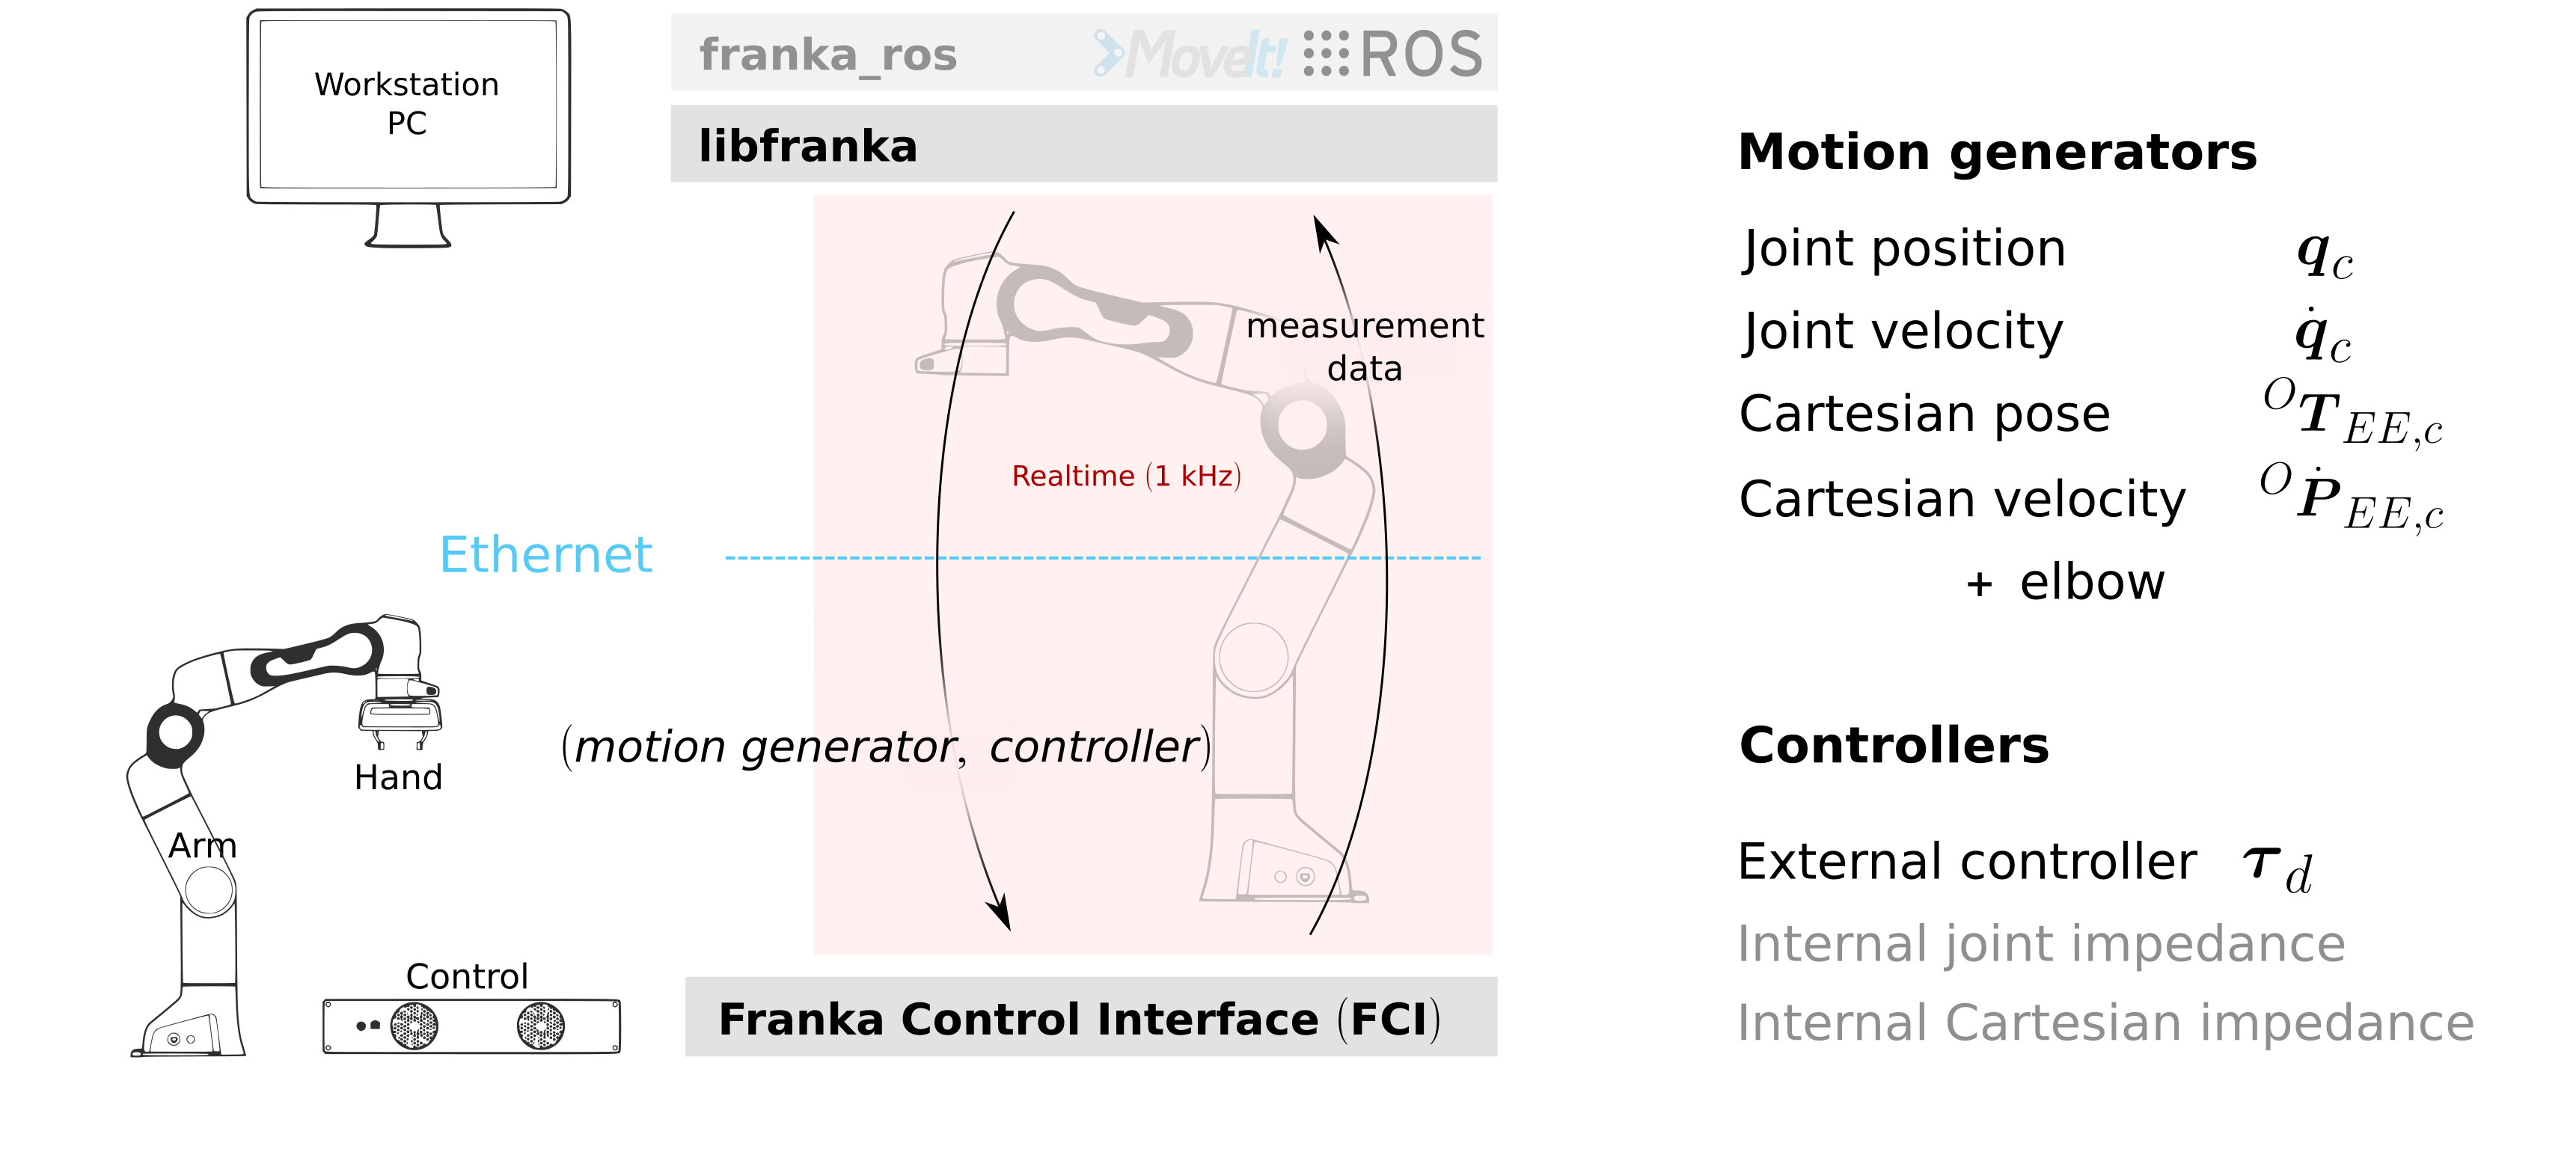
\includegraphics[width=\linewidth]{rt-interfaces.png}
	\caption{Control interface schematic.}
	\label{fig:interface} 
\end{figure}

\section{Control} \label{sec:control}
\subsection{Control Overview}
The control framework of the project is shown in Figure \ref{fig:framework}. The MPC controller calculates the optimal trajectory to the target position, based on a linear model of the robot. Reference commands in the form of velocity signals based on this trajectory are then sent to the robot. The Franka Emika control interface implements an inner feedback loop using a PI controller. Because of this, it is reasonable to assume that the joints configure themselves as commanded, and therefore an open-loop control approach is possible. However, an external interference may cause the robot to be in a different joint configuration than commanded. When this occurs, it is essential that the MPC controller receives information about the robot’s new position, in order to generate a new trajectory. This requires a feedback control loop shown by the dotted line in Figure \ref{fig:framework}.

% Update this figure with torques also being fed back
\begin{figure}[b]
	\centering
	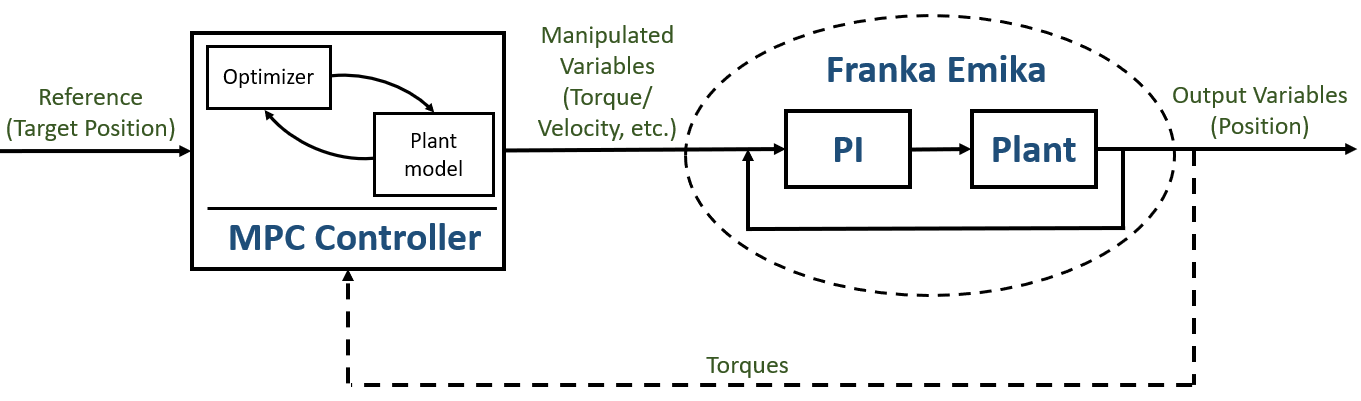
\includegraphics[width=1\columnwidth]{MPC4.png}
	\caption{The Control Framework}
	\label{fig:framework} 
\end{figure}

\subsection{MPC}
MPC uses a discretized model of the plant to predict the future trajectory and solves an online optimization problem to select the best sequence of control actions that drives the predicted output to the reference. The controlled variables for the plant are defined as:
\begin{equation}
    z(k) = \zeta(k).
    \label{eq:def_controlled_variable}
\end{equation}
Based on the plant discretized model \eqref{eq:DiscretizedLinearModel}, future trajectories can be predicted provided different control signals. 
The future control signals and the corresponding future controlled variables in $N$ time steps are defined as:
\begin{equation}
    \mathcal{U} = [u^T(k), u^T(k+1), ..., u^T(k+N-1)]^T,
\end{equation}
\begin{equation}
    \mathcal{Z} = [z^T(k+1), z^T(k+2), ..., z^T(k+N)]^T,
\end{equation}
where $N$ is the prediction horizon, and $k$ denotes the current step.
In this application, $N$ remains constant at 25, therefore the prediction is always broken down into 25 steps. The control horizon is the same, therefore commands are generated for every step. Because the prediction horizon remains constant, the sample time varies with elapsed time, as shown in \eqref{eq:sample_period}. Thus, the prediction is broken down into increasingly smaller, more precise steps as the target is approached, therefore increasing accuracy.

\subsection{Cost Function}
To find the best-predicted path, the optimizer then evaluates the cost function $J$ for each predicted trajectory. The optimal trajectory is one in which joint velocity, joint acceleration and control inputs along the path are minimised. Consider the quadratic cost function $J$ as
\begin{equation}
    \label{eq:costFunc}
    J_k(\mathcal{U}) = \sum_{i=k+1}^{k+N}||x(i)||^2_{Q(i)}
    + \sum_{i=k}^{k+N-1}||u(i)||^2_{R(i)},
\end{equation}
where $Q$, $R$ are weight matrices\footnote{$||a||^2_W = a^TWa$ for a positive semidefinite weight matrix $W$.}. The weighting matrices were chosen to be constant and equal for each of the joints; penalizing states with $\Tilde{Q}$, and input with $\Tilde{R}$:
\begin{equation}
    \Tilde{Q} = \begin{bmatrix}0 & 0 & 0 \\ 0 & 1 & 0 \\ 0 & 0 & 1\end{bmatrix}, \quad \Tilde{R} = 0.001.
\end{equation}
Assembly of these result in the system weighting matrices
\begin{equation}
    Q = \mathrm{blkdiag}([\Tilde{Q},\dots, \Tilde{Q}]), \quad 
    R = \mathrm{blkdiag}([\Tilde{R}, \dots \Tilde{R}]),
\end{equation}
with the dimensions $Q\in \mathbb{R}^{3d\times 3d}$ and $R\in \mathbb{R}^{d\times d}$.
A possible improvement to the control could be to punish the states differently when nearing the goal state, i.e., have time-dependent weighting matrices. 

%Consider the general cost function presented in the previous section. Now, the reference $r(i)$ does not need to be defined at every sample \cite{MPC2019}. This suits the application of point-to-point trajectory generation as it may be desirable to leave the entire trajectory generation to the optimizer. The cost function can therefore be simplified as follows.

\subsection{Constraints}
The equations below list the constraints the system and model are subject to. Physical limitations of the robot, such as joint state constraints and control signal below, are defined by the manufacturer in the documentation \cite{frankadocs}.
\subsubsection{Physical Constraints on Joints} \eqref{eq:constr_predicted_states} shows the maximum and minimum limits on the controlled variables, i.e. joint angles, velocities and accelerations,
\begin{equation}
    \begin{split}
        [x_{min}^1, \dots,& x_{min}^d]^T \leq x(i) \leq [x_{max}^1, \dots, x_{max}^d]^T, \\
        & \quad\quad\quad\quad\quad\quad\quad k+1 \leq i \leq k+N, \\
        \textrm{where} \quad\quad\quad &\\ 
        x_{max}^j & = [q_{max}^j, v_{max}^j, a_{max}^j], \\ 
        x_{min}^j & = [q_{min}^j, v_{min}^j, a_{min}^j], \quad 1\leq j \leq d.
    \end{split}
    \label{eq:constr_predicted_states}
\end{equation}

\subsubsection{Constraints on Control Signals}
The following equation \eqref{eq:constr_umax} limits the control signals of the system, modeled as jerk,
\begin{equation}
    |u(i)|\leq [u_{max}^1, \dots, u_{max}^d]^T, k \leq i \leq k+N-1.
    \label{eq:constr_umax}
\end{equation}

\subsubsection{Variable Relationship}
Related to the state variable $\zeta$ through the variable transformation performed in \eqref{State_Vari_Trans} and a definition in \eqref{eq:def_controlled_variable}. A variable relation between $x$ and $z$ is provided as, 
\begin{equation}
    \label{eq:constr_variablechange}
    x(i) = z(i)+\frac{1}{h}\Gamma_1u(i), \quad k+1\leq i\leq k+N.
\end{equation}

\subsubsection{Final State}
\eqref{eq:constr_rf} is the constraint on the controlled variable at the final time in the prediction horizon, i.e., the goal state. 
\begin{equation}
    x(k+N) = r_f.
    \label{eq:constr_rf}
\end{equation}

Given the initial state $x(k)$ of the system in each sample $k$, the following optimization problem is solved in the MPC:
\begin{equation}
    \begin{split}
    \label{eq:optimization}
        &\min_{\mathcal{U}} J_k(\mathcal{U})\\
        &\text{subject to} \,\,\eqref{eq:constr_predicted_states}- \eqref{eq:constr_rf}
    \end{split}
\end{equation}
Therefore, a complete MPC Controller is constructed. The validation of the optimization problem \eqref{eq:constr_rf} is discussed in the Appendix \ref{apx:proof}.

% refer to the part 'point-to-point planning' of the paper
\subsection{Trajectory Interpolation}
In the implementation, solving the optimization problem simultaneously for all joints is highly computationally expensive. An alternative is to perform trajectory planning on each joint separately (viable due to the decoupling of the joints). This kind of implementation has been proven to work well in the program, taking only a few milliseconds to solve the optimization problem for all joints. However, as the robot requires control commands every millisecond, the trajectory calculation still has a high probability of missing the deadline. To compensate for this, the trajectory obtained previously is considered valid until the calculation of a new trajectory is completed. A linear trajectory interpolation is applied to the reference points at each control period. Assuming T is a vector of increasing time constant, and $R_f$ is a matrix of the corresponding reference points
\begin{equation}
    T =[t_1,t_2,\dots,t_n],
\end{equation}
\begin{equation}
    R_f=[r(1),r(2),\dots,r(n)],
\end{equation}
 the continuous time reference point $r_c$ is defined using a linear interpolation such that
\begin{equation}
    r_c(t) = r(k) + \frac{r(k+1)-r(k)}{t_{k+1}-t_k}(t-t_k),\quad t_k\leq t<t_k+1.
\end{equation}

\section{Simulation}\label{sec:simulation}
To verify the control design proposed in the previous section and the generated CVXGEN code, a simulation of the system was made. A simple Matlab Simulink model was constructed, which can be seen in Figure \ref{fig:sim_model}. Start pose ($x_1=0$ rad), reference pose ($x_1=\pi/4$ rad) and sample time $h$ are fed to the calculation block. The calculated input is fed back through a state space block. The simulation results are shown in Fig. \ref{fig:sim_result}. The simulated joint arrived at the target position accurately at the given time of 1 second. The velocities close to starting and reference points are small, which indicates a soft motion. The simulation result provides a good instruction of ideal graphs to be obtained in the following experiment.   

The simulation code is presented in the git repository folder \texttt{src/simulation/}.\cite{gitrepo} 

\begin{figure}
    \centering
    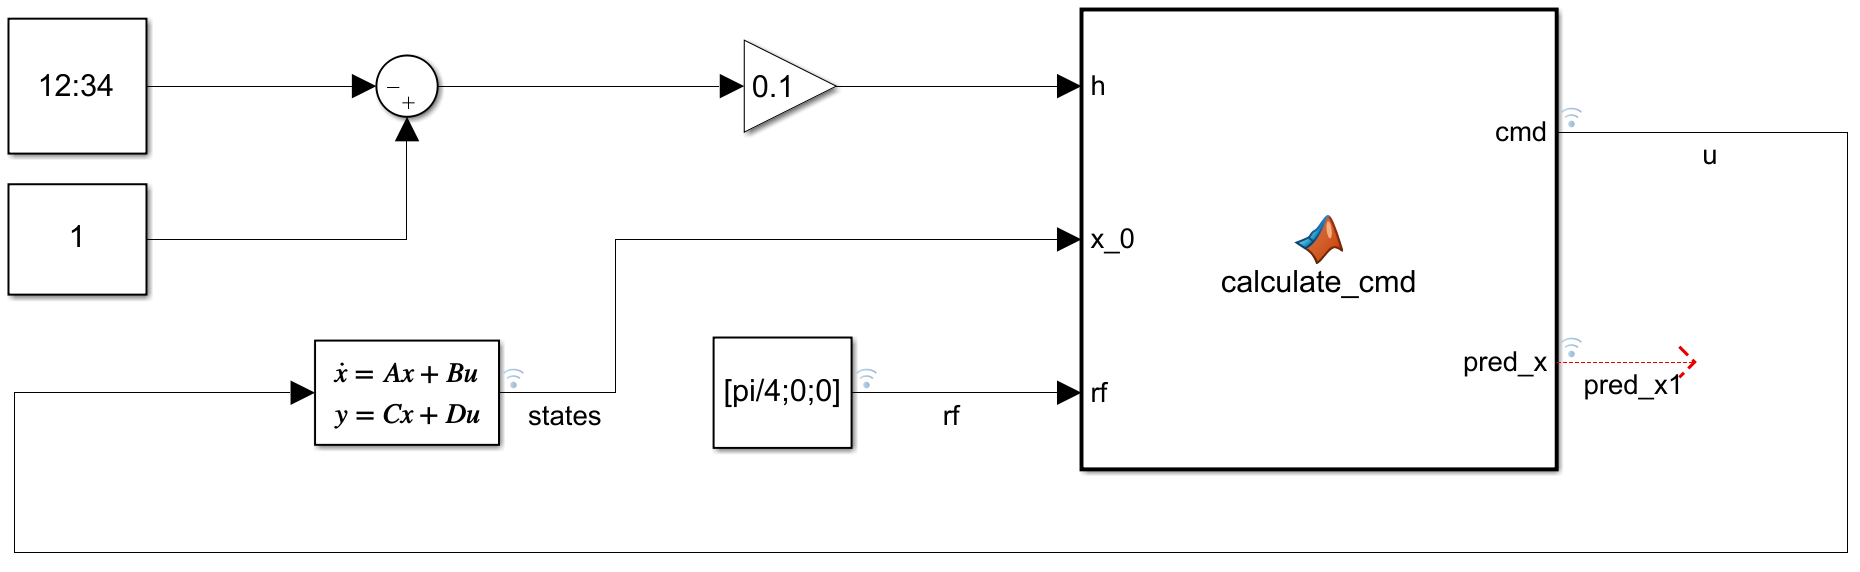
\includegraphics[width=\linewidth]{simulink_model.png}
    \caption{Simulink model for control and code verification.}
    \label{fig:sim_model}
\end{figure}

\begin{figure}
    \centering
    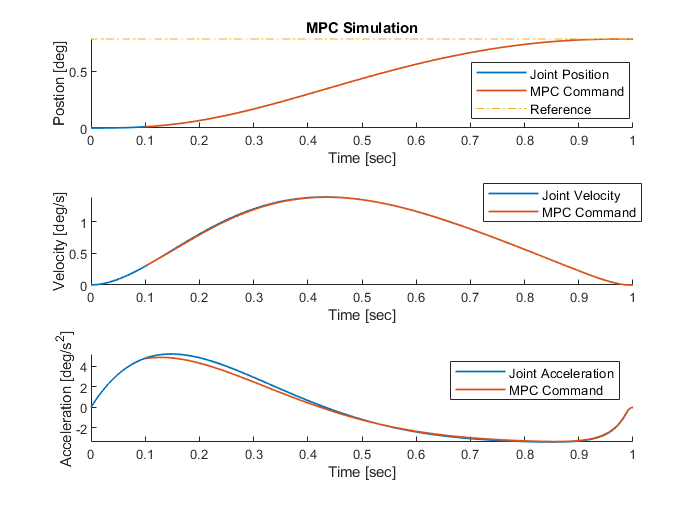
\includegraphics[width=\linewidth]{simfig.png}
    \caption{MPC simulation results showing arrival at reference pose.}
    \label{fig:sim_result}
\end{figure}

\section{Experiment}\label{sec:experiment}
\subsection{Implementation}
The code structure of this work is shown in Figure \ref{fig:code_structure}. There are two threads for control purposes, in addition to the \texttt{main}-thread.

The MPC thread initializes the CVXGEN-code (further described below) and runs the solver every 10 ms. The reference states of a new trajectory are calculated joint by joint and saved in the variable monitor. The variable monitor is set up to avoid conflicts that might appear when to read or write the same address in the memory at the same time. This monitor is implemented using a mutex lock provided by the class \texttt{pthread}.

The communication thread executes at a frequency of 1 kHz as required by the real-time control interface provided by Franka. As stated earlier, the computational time of optimization in MPC usually exceeds the limitation of one millisecond. It is therefore necessary to construct the program in a multi-thread structure. This was done using the \texttt{pthread} class in C++. The communication thread reads the reference points from the optimization result of the MPC. These reference points have a lower resolution than one millisecond, and linear interpolation of the command is therefore executed before being sent to the robot. 
State feedback from the robot is used to read externally applied torque. If the torque exceeds a predefined threshold, reference tracking is disabled and manual force control is enabled. Force control permits the user to push the robot in the desired direction. After a period of time without disturbance, the robot returns to reference tracking and follows the latest MPC-generated trajectory.

The communication thread also handles user input. At the start of the script, the user can enter a start and end position. At any moment during run-time, the motion can be canceled in the terminal or by pressing the robots stop button.

The main thread initializes the above control threads and prints accuracy results in the terminal at the end of the task.

\begin{figure}
	\centering
	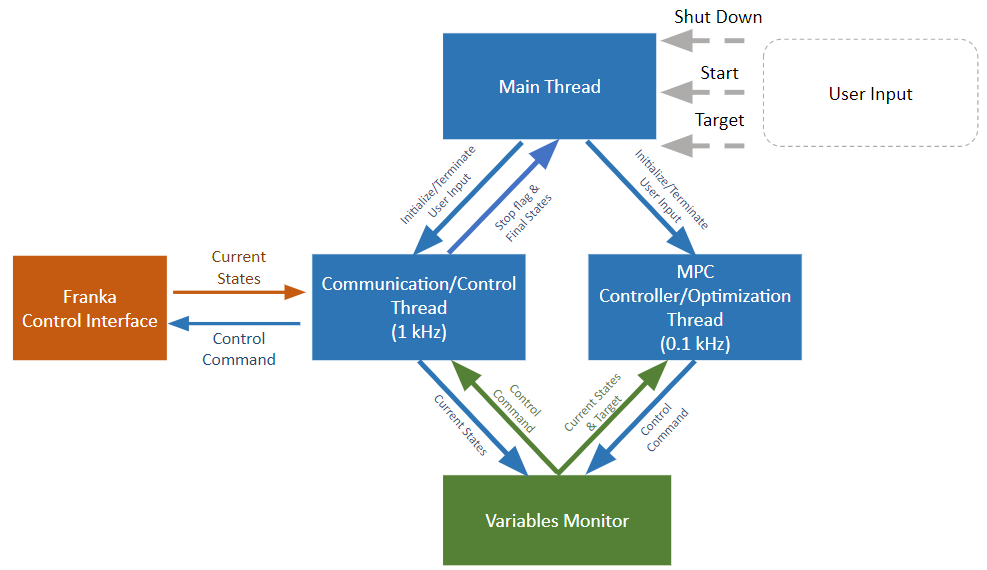
\includegraphics[width=1\columnwidth]{code_structure.PNG}
	\caption{The code implementation structure}
	\label{fig:code_structure} 
\end{figure}

\subsubsection{CVXGEN}
CVXGEN is a program that generates small, fast \texttt{C}-code that solves convex optimization problems \cite{cvxgen}. It is used in this project to generate the trajectory, i.e., time-stamped joint states and system input, i.e., torque. By including the CVXGEN-generated code in the code structure of the control interface \texttt{libfranka}, the solution to the optimization problem could be obtained by providing parameters from the robot, using the CVXGEN function \texttt{solve()} and reading the optimized variables. The CVXGEN code is presented in the git repository folder \texttt{src/cvxgen/}.\cite{gitrepo} 

\subsection{Point-To-Point Experiment}
% Add trajectory experiment
To test the implementation described in the section above, the robot was set up to perform two separate motions. The reference signal to the robot was a velocity command.
\begin{itemize}
    \item \textbf{Motion A:} Pick-up-motion starting low and moving up and back. The robot was undisturbed during this motion. The time limit was 5 seconds.
<<<<<<< HEAD
    \item \textbf{Motion B:} Horizontal translation. The robot was subjected to a disturbance by being pushed out of trajectory by a human user. This action lasted for 1.38 s. The time limit was 5 seconds including disturbance.
=======
    \item \textbf{Motion B:} Horizontal translation. The robot was subjected to a disturbance by being pushed out of trajectory by a human user. This action lasted for 1.38 s. The time limit was 5 seconds (including disturbance).
>>>>>>> f604414f387b8ccc24728783384143945bbc4ad1
\end{itemize}

\section{Results} \label{sec:Results}
A visualization of a sample of generated position trajectories (every one second) can be seen in Figure \ref{fig:trajectory_result}. The plot confirms that the MPC functions as in the previous simulation. However, small errors appeared on the starting point of some trajectories. They possibly resulted from the mismatch between the initial states sent to MPC and the real initial states.

\begin{figure}
    \centering
    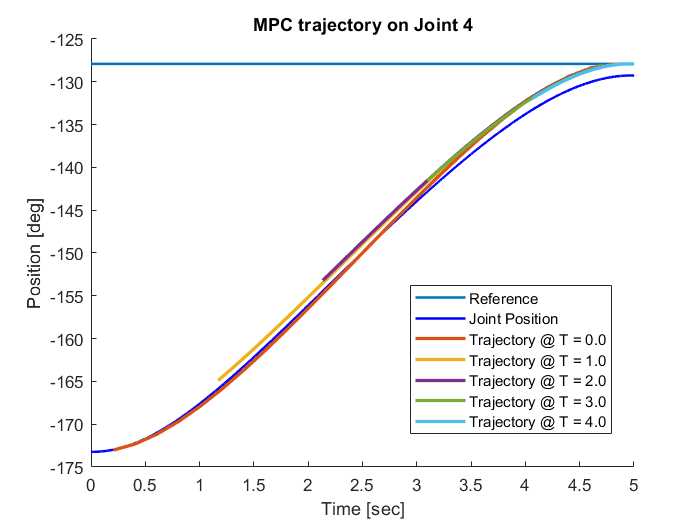
\includegraphics[width=\linewidth]{MPC_trajectory_J4.png}
    \caption{The MPC-generated trajectories on joint 4 during Motion A.}
    \label{fig:trajectory_result}
\end{figure}

The plot of Motion A can be seen in Figure \ref{fig:joint_result_wo_perturbation}. The graphs show the MPC-generated command, of which only the velocity is sent to the robot and the actual joint states. The actual acceleration, which has small oscillations, is controlled by the built-in PI controller of the robot. Table \ref{tab:joint_result_wo_perturbation} presents this motion's reference and achieved joint positions.

\begin{figure}
    \centering
    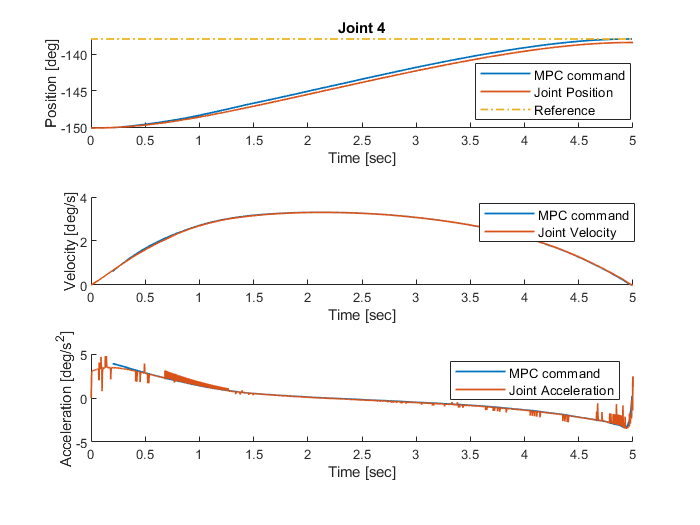
\includegraphics[width=\linewidth]{result_without_perturbation_Joint4.png}
    \caption{Motion A: Angular position, velocity and acceleration plots of joint 4 without perturbation.}
    \label{fig:joint_result_wo_perturbation}
\end{figure}

\begin{table}[t]
	\centering
	\caption{Motion A: Reference and achieved position without perturbation.}
	\label{tab:joint_result_wo_perturbation}
	\begin{tabular}{crr} % (l)eft, (r)ight and (c)enter indentation
		\toprule
		Joint number & Distance & Error \\ 
		 &  [deg] & [deg] \\ 
        \midrule
		1 & -43.82   & 1.39609    \\ 
		2 & 64.04    & 0.04900   \\ 
		3 & -31.84   & 0.44157    \\ 
		4 & 12.21    & -0.47929  \\ 
		5 & 24.74    & -0.39199  \\
		6 & 45.81    & 0.21843   \\ 
		7 & -107.04  & -0.04494   \\ 
        \bottomrule 
	\end{tabular}
\end{table}

The plot Motion B can be seen in Figure \ref{fig:joint_result_w_perturbation}. The start- and end-time of the perturbation is marked with a dotted, red line. When the robot is under perturbation, it sends current states to MPC as feedback to calculate new trajectory to target position. Table \ref{tab:joint_result_w_perturbation} presents this motion's reference and achieved joint positions. 

<<<<<<< HEAD
The remaining angular position error was found to be dependent on the moving distance of the joint, if not given sufficient time for the motion. In other words, a perturbation did not affect accuracy.
=======
The remaining angular position error was found dependent on the moving distance of the joint, if not given sufficient time. In other words, a perturbation did not affect accuracy.
>>>>>>> f604414f387b8ccc24728783384143945bbc4ad1

\begin{figure}
    \centering
    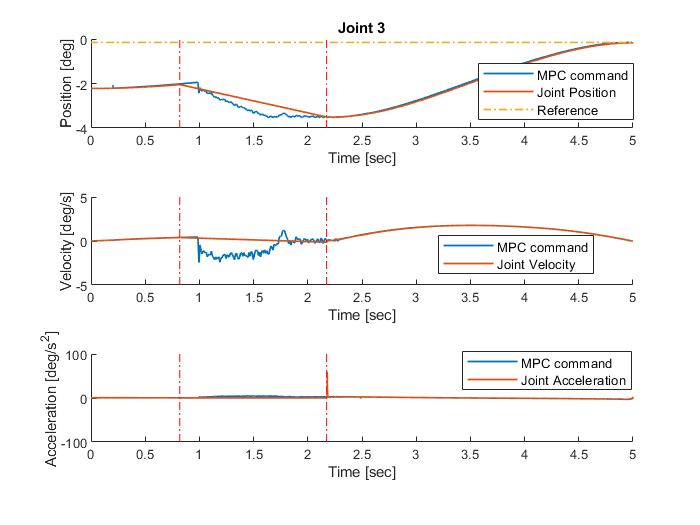
\includegraphics[width=\linewidth]{result_under_perturbation_Joint3.png}
    \caption{Motion B: Angular position, velocity and acceleration plots of joint 3 with perturbation.}
    \label{fig:joint_result_w_perturbation}
\end{figure}

\begin{table}[t]
	\centering
	\caption{Motion B: Moved distance and resulting position error with perturbation.}
	\label{tab:joint_result_w_perturbation}
	\begin{tabular}{crr} % (l)eft, (r)ight and (c)enter indentation
		\toprule
		Joint number & Distance & Error \\ 
		 &  [deg] & [deg] \\ 
        \midrule
		1 & 0.49    & -0.03755 \\
		2 & -13.48  & -0.08306\\
		3 & 2.37    & -0.01969 \\
		4 & 39.32   & -0.87068 \\
		5 & 1.77    & -0.01486 \\
		6 & -52.31  & 0.00137 \\  
        \bottomrule 
	\end{tabular}
\end{table}

The control code of the project is presented in the git repository folder \texttt{src/examples}.\cite{gitrepo} For instructions on how to run the code on any PC where the Franka control interface \texttt{libfranka} is installed, see the \texttt{README.md} file of the git repository.

\section{Discussion} \label{sec:Conclusion}

In this project, an MPC-based real-time trajectory planning methodology is implemented on a 7 DoF robot Franka Emika Panda. Starting from modeling each joint of the robot arm under joint coordinates, a linear model of the robot dynamics is derived and applied to the prediction of future motion in an MPC controller. 

At the time of the project start, a source of confusion was what commands should be sent to the robot. As there is already an inner controller, the target states (position, velocity, etc.) are sent to the robots rather than jerk input signals. The CVXGEN code solves the optimization problem of MPC, and the reference points can be sent to Panda to track the trajectory.

As seen in Figures \ref{fig:joint_result_wo_perturbation} \& \ref{fig:joint_result_w_perturbation}, the final velocity command tracking of the robot is accurate, and therefore the design choice of an open-loop control approach is validated. 
The accuracy shown in \ref{fig:joint_result_w_perturbation} also validates the method used to handle external perturbations. A new trajectory is generated whenever the robot senses perturbation, and it guarantees the robot to arrive at the target position at a given time. However, it was found that if the perturbation time nears or exceeds the maximum allowed time, the MPC fails to generate a valid trajectory and invalid commands may be sent to the robot.

In the final implementation of the MPC, a prediction horizon of 25 is used. When compared to a prediction horizon of 10 (as was initially trialed), it was evident that the better value gave much more excellent performance. Higher control accuracy is achieved with an acceptable computation time increase. 

The weight matrices used in the cost function were determined by previous work.\cite{MPC2019} There was no evidence encountered to indicate that these weightings should be considered invalid. However, there is a potential to investigate the influence of different weight matrices. 


A multi-thread code structure is used in this project to handle the conflicts between the requirement of high control frequency and the limitation of high computational costs in optimization. When any external disturbance appears, the torque sensors trigger the closed-loop control, and the real-time trajectory planning method generates a new trajectory to correct its direction towards the target position. Implementing both the closed-loop and the open-loop control methods together proved difficult. Particular attention had to be paid to the initial states of the MPC, as they are different in open-loop control and closed-loop control. In the open-loop control, the initial states are obtained from the linear extrapolation. In the closed-loop control, the robot sends current states to MPC as initial states.

% efficiency
Though a high accuracy control performance has been achieved, the efficiency of motion is unsatisfying. Trajectories generated joint-wise are not efficient for point-to-point motion, i.e., the end effector moves in an arc rather than a straight line. This is because the MPC is designed in joint space. The limitation could be overcome if Cartesian space is used. This would require inverse kinematics.

% possible applications
There is lots of potential for this project to be extended into the industrial field, as it allows smooth interaction between the user and the robot. For example, it can be easily programmed to perform a repetitive task and is also simple to adjust if necessary. On top of this, the possibility to interact with the robot while it is running is an excellent safety feature, because it can be used to avoid collisions.

% Prints cited references
\printbibliography
\newpage
\section*{Appendices}
\appendix

\section{Cost Function Validation} \label{apx:proof}
In this section, a proof on the the existence of global minimum for the cost function $J$ \eqref{eq:costFunc} under constraints \eqref{eq:constr_predicted_states}- \eqref{eq:constr_rf} is presented to validate the proposed optimization problem \eqref{eq:optimization}.

The variables in cost function $J$ \eqref{eq:costFunc} are linearly dependent by the relationship in \eqref{eq:discr-time_model}. Therefore, the cost function $J$ has $N+1$ linearly independent variables
\begin{equation}
    x_{new}(k) = [x(k), u(k), ..., u(k+N-1)]^T \in S \subset \mathbb{R}^{N+1}
\end{equation}

The objective function, i.e., the cost function $J$ is continuous, and the set $S$ is compact by the constraints in \eqref{eq:constr_predicted_states} and \eqref{eq:constr_umax}. Therefore, by Weierstrass Theorem, a minimum exists in the problem \eqref{eq:constr_rf}.

Because the cost function $J$ is constructed by convex quadratic terms, the cost function $J:S \to \mathbb{R}$ is convex. Thus the local minimum is the global minimum.


\end{document}





